\documentclass[11pt,a4paper]{article}
\usepackage[T1]{fontenc}
\usepackage[utf8]{inputenc}
\usepackage[french]{babel}
\usepackage{lmodern}
\usepackage[margin=2.2cm]{geometry}
\usepackage{amsmath,amssymb}
\usepackage{booktabs}
\usepackage{array}
\usepackage{graphicx}
\usepackage{float}
\usepackage{needspace}
\usepackage{enumitem}
\usepackage[skins,breakable]{tcolorbox}
\usepackage[font=small,labelfont=bf,labelsep=period]{caption}
\frenchsetup{StandardItemLabels=true}
\usepackage[hidelinks]{hyperref}

\setlength{\emergencystretch}{3em}
\setlist{itemsep=2pt,topsep=4pt}
\newcommand{\code}[1]{\texttt{#1}}
\newcommand{\shift}{\mathrm{shift}}
\definecolor{bleu}{HTML}{2a78d6}
\definecolor{orange}{HTML}{eb6834}
\definecolor{vert}{HTML}{1baf7a}
\newtcolorbox{retenir}{breakable,enhanced,colback=bleu!5,colframe=bleu!70,boxrule=0.6pt,arc=2pt,
  left=6pt,right=6pt,top=4pt,bottom=4pt,title=À retenir,fonttitle=\bfseries\small,coltitle=white}
\newtcolorbox{exemple}[1]{breakable,enhanced,colback=orange!4,colframe=orange!75,boxrule=0.6pt,arc=2pt,
  left=6pt,right=6pt,top=4pt,bottom=4pt,title={Exemple : #1},fonttitle=\bfseries\small,coltitle=white}
\newtcolorbox{hypo}[1]{breakable,enhanced,colback=vert!5,colframe=vert!75,boxrule=0.6pt,arc=2pt,
  left=6pt,right=6pt,top=4pt,bottom=4pt,title={#1},fonttitle=\bfseries\small,coltitle=white}

\title{Jouer aux échecs avec des matrices\\[4pt]
\large Du plateau au GPU : la théorie pas à pas, les expériences et les pistes\\[2pt]
\normalsize Rapport de synthèse du projet \code{chess-gpu}}
\author{Branche \code{claude/zen-pasteur-vjg9yx}}
\date{25 novembre 2026}


\begin{document}
\maketitle

\begin{abstract}
Ce projet part d'une idée simple. Une position d'échecs est une matrice d'entiers, un coup est une
autre matrice, et jouer un coup revient à les multiplier. Si tout s'écrit ainsi, une carte
graphique, conçue pour multiplier des matrices en masse, doit pouvoir explorer des millions de
positions par seconde. Ce rapport reprend le projet depuis le début. Chaque notion part d'un
exemple sur l'échiquier et aboutit à son écriture formelle. Il traite dans l'ordre le codage des
positions, les déplacements vus comme des décalages, les coups vus comme des matrices
$64\times64$, l'inversion et l'analyse rétrograde, le calcul par lots sur GPU, puis la recherche du
meilleur coup vue comme une convergence d'intervalles. Les expériences sont résumées en cinq fils
conducteurs. Le GPU compte les positions 157 fois plus vite que Stockfish sur un cœur, mais la
force de jeu dépend surtout de la profondeur atteinte, donc de l'élagage et du tri des coups. Le
rapport se termine par sept hypothèses pour la suite, chacune avec son protocole de mesure.
\end{abstract}

\tableofcontents

\section*{Comment lire ce rapport}
\addcontentsline{toc}{section}{Comment lire ce rapport}
Chaque partie montre d'abord une position sur l'échiquier, puis écrit la même chose en matrices.
La complexité augmente d'une partie à l'autre. On passe d'une case à une pièce, puis à un coup, à
une partie entière, à des millions de positions, et enfin à la recherche du meilleur coup. Trois
sortes d'encadrés ponctuent le texte.
\begin{itemize}
\item Les encadrés \textcolor{orange}{\textbf{Exemple}} donnent un cas chiffré, calculé par le
moteur.
\item Les encadrés \textcolor{bleu}{\textbf{À retenir}} résument une partie en quelques lignes.
\item Les encadrés \textcolor{vert}{\textbf{Hypothèse}} proposent une piste pour la suite.
\end{itemize}
Le script \code{gen\_figures.py}, placé à côté de ce fichier, appelle directement
\code{src/matrix\_chess} pour produire les figures et les exemples chiffrés. Une seule courbe
reprend des valeurs publiées ailleurs, la perte par profondeur de la partie~7, tirée du rapport de
l'incrément~1. Les résultats de matchs cités dans le texte viennent des rapports des incréments.

% =====================================================================================================
\section{Le parcours en une page}

Le projet a avancé en quatre étapes. Chacune a répondu à une question et en a soulevé une autre.

\begin{table}[H]
\centering\small
\begin{tabular}{>{\raggedright\arraybackslash}p{2.4cm}>{\raggedright\arraybackslash}p{5.1cm}>{\raggedright\arraybackslash}p{7.2cm}}
\toprule
Étape & Question & Réponse\\
\midrule
Phase 1, février & Un réseau qui imite les grands maîtres joue-t-il bien ? &
Non. Il trouve le coup du maître une fois sur quatre, mais ne suit aucun plan. Son niveau se situe
entre 840 et 950 Elo.\\
Théorie, de février à juillet & Peut-on écrire toutes les règles en matrices ? &
Oui. Les déplacements sont des décalages, les coups sont des matrices $T$, et l'inversion est
affine. Comparé à \code{python-chess}, le moteur ne présente aucune divergence.\\
Incrément 1, novembre & Le GPU va-t-il plus vite que Stockfish ? Peut-on écrire l'alpha-bêta en
calcul matriciel ? &
Le GPU compte 157 fois plus de positions par seconde. La force de jeu, elle, dépend de la
profondeur atteinte. L'alpha-bêta par lots, exact, marque 7,5/14 contre Stockfish dans ses
conditions de calibration.\\
Incrément 2, novembre & Où nos coups perdent-ils de la valeur ? Le tri et la pendule rendent-ils
le moteur plus fort ? &
Les parties se perdent entre les coups 11 et 20. Le moteur de l'incrément 2 gagne $+127$ Elo
contre celui de l'incrément 1, sur 200 parties.\\
\bottomrule
\end{tabular}
\caption{Les quatre étapes du projet. Chaque étude a son dossier daté dans \code{docs/etudes/}.}
\end{table}

Le calcul matriciel donne un débit très élevé. L'essentiel du travail a consisté à transformer ce
débit en profondeur de recherche. Les parties~2 à~5 expliquent d'où vient le débit. La partie~6
montre comment on le convertit en profondeur. Les parties~7 et~8 disent ce que les expériences en
ont appris et ce qu'il reste à essayer.

% =====================================================================================================
\section{Une position est une matrice}

\subsection{Coder les pièces par des entiers}
On numérote les six sortes de pièces : pion $1$, cavalier $2$, fou $3$, tour $4$, dame $5$,
roi $6$. Une pièce blanche garde son nombre, une pièce noire prend le signe moins, et une case vide
vaut $0$. Le plateau devient une matrice $B\in\mathbb{Z}^{8\times8}$. La ligne $i=0$ est la
rangée~8, en haut, du côté des noirs. La colonne $j=0$ est la colonne~a.

\begin{figure}[H]
\centering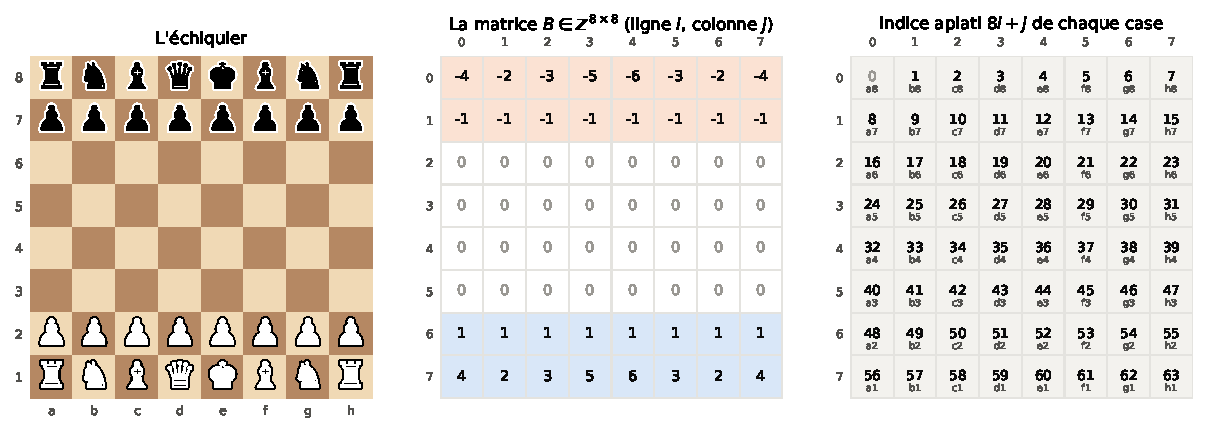
\includegraphics[width=\textwidth]{figs/plateau.pdf}
\caption{La position de départ, sa matrice $B$ et l'indice de chaque case. Les cases bleues sont
positives (pièces blanches), les cases orange sont négatives (pièces noires).}
\end{figure}

La matrice se lit comme l'échiquier. Sa première ligne, $(-4,-2,-3,-5,-6,-3,-2,-4)$, donne la
rangée~8 des noirs dans l'ordre tour, cavalier, fou, dame, roi, fou, cavalier, tour. Les quatre
lignes centrales sont nulles. Le signe indique la couleur, la valeur absolue indique la pièce.

\subsection{Aplatir en un vecteur}
Pour multiplier par une matrice, on range les 64 cases dans un vecteur $b\in\mathbb{Z}^{64}$, ligne
après ligne. La case $(i,j)$ reçoit l'indice $8i+j$. Ainsi a8 vaut~0, h8 vaut~7, a1 vaut~56 et h1
vaut~63.
\[ b = (b_0,\dots,b_{63}),\quad b_{0} = -4\ (\text{a8}),\quad b_{60} = +6\ (\text{e1}),\quad b_{52} = +1\ (\text{e2}),\quad b_{36} = 0\ (\text{e4})
\unskip \]
C'est l'ordre que \code{numpy} utilise pour \code{B.reshape(64)}, si bien qu'aucune conversion n'est
nécessaire.

\begin{retenir}
Une position est un vecteur $b$ de 64 entiers. Le signe d'une valeur donne la couleur, sa valeur
absolue donne la pièce. Le trait, les droits de roque et la case de prise en passant sont stockés à
part, dans l'objet \code{Game}.
\end{retenir}

% =====================================================================================================
\section{Un déplacement est un décalage}

\subsection{Le décalage, opération de base}
Plaçons un 1 sur la case d4 et des 0 partout ailleurs. On obtient une matrice $P$ qui marque une
pièce. Décaler $P$ d'une ligne vers le haut marque la case d5. Décaler $P$ de deux lignes vers le
haut et d'une colonne vers la droite marque e6, soit un saut de cavalier. On note
$\shift(P, d_r, d_c)$ le décalage de $d_r$ lignes et de $d_c$ colonnes, où des zéros entrent par
le bord.

\begin{figure}[H]
\centering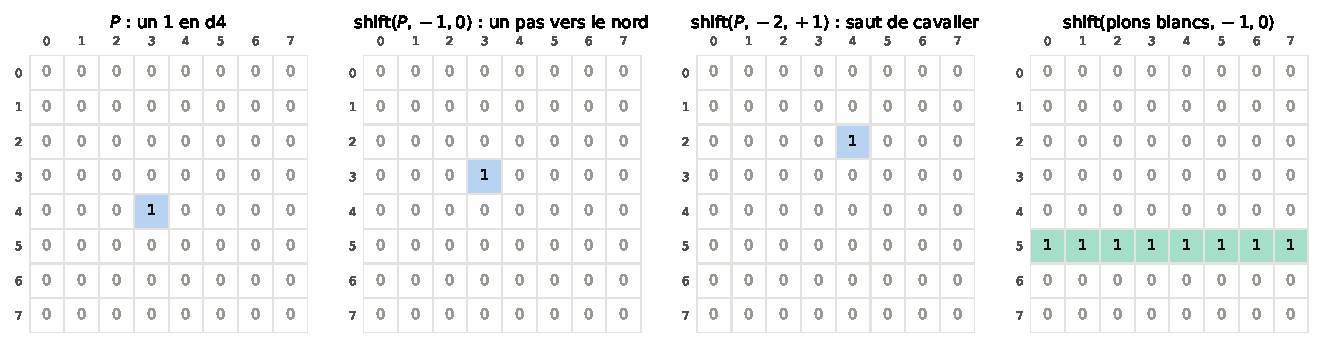
\includegraphics[width=\textwidth]{figs/decalage.pdf}
\caption{Le décalage déplace tous les 1 en même temps. À droite, un seul décalage fait avancer les
huit pions blancs.}
\end{figure}

Le décalage est lui-même un produit de matrices. Soit $S_d$ la matrice $8\times8$ qui porte des 1
sur sa $d$-ième diagonale. Alors
\[ S_{-1} = \begin{pmatrix}0 & 1 & 0 & 0 & 0 & 0 & 0 & 0 \\ 0 & 0 & 1 & 0 & 0 & 0 & 0 & 0 \\ 0 & 0 & 0 & 1 & 0 & 0 & 0 & 0 \\ 0 & 0 & 0 & 0 & 1 & 0 & 0 & 0 \\ 0 & 0 & 0 & 0 & 0 & 1 & 0 & 0 \\ 0 & 0 & 0 & 0 & 0 & 0 & 1 & 0 \\ 0 & 0 & 0 & 0 & 0 & 0 & 0 & 1 \\ 0 & 0 & 0 & 0 & 0 & 0 & 0 & 0\end{pmatrix},\qquad \mathrm{shift}(M, d_r, d_c) = S_{d_r}\, M\, S_{d_c}^{\top}
 \]
Le script vérifie cette égalité pour les 16 décalages utiles, soit les 8 directions du roi et les
8 sauts du cavalier. Le reste du moteur repose sur deux conséquences.
\begin{itemize}
\item \textbf{Les bords ne demandent aucun test.} Ce qui sort du plateau sort de la matrice et
disparaît. Aucun \code{if} ne vérifie qu'une case existe.
\item \textbf{Un décalage agit sur toutes les pièces en même temps.} La figure le montre avec les
pions. Il agit de la même façon sur des millions de plateaux, ce que le GPU exploitera.
\end{itemize}

\subsection{Le roi : une convolution}
Le roi avance d'une case dans l'une des huit directions. Ses destinations forment donc l'union de
huit décalages de $P$. Écrite comme une somme pondérée, cette union est une convolution par le
noyau
\[ K_{\text{roi}} = \begin{pmatrix}1 & 1 & 1 \\ 1 & 0 & 1 \\ 1 & 1 & 1\end{pmatrix}
\unskip \]
\begin{figure}[H]
\centering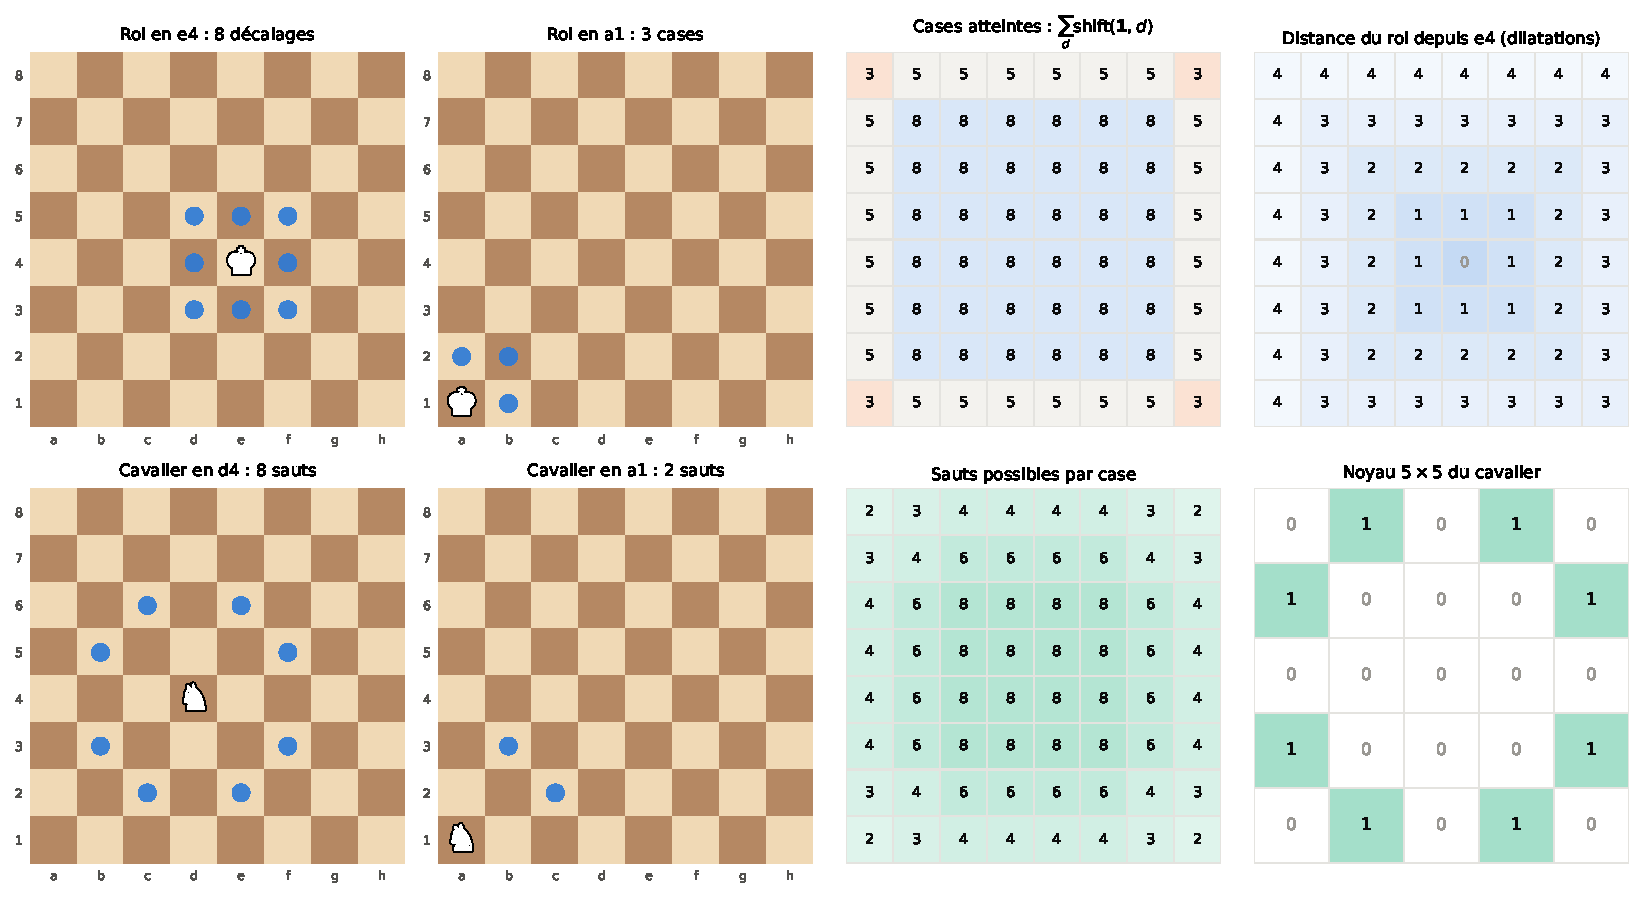
\includegraphics[width=\textwidth]{figs/roi_cavalier.pdf}
\caption{En haut, le roi. Au centre, il atteint 8 cases. Dans le coin, les décalages qui sortent du
plateau s'annulent et il en reste 3. Appliqués à un plateau rempli de 1, les huit décalages
comptent les cases atteignables depuis chaque case. En répétant la dilatation, on obtient la
distance du roi, c'est-à-dire la distance de Chebyshev $\max(|\Delta i|,|\Delta j|)$. En bas, le
cavalier. Ses huit sauts forment une convolution par un noyau $5\times5$.}
\end{figure}

\subsection{Les pièces glissantes : une propagation}
La tour, le fou et la dame avancent jusqu'à la première pièce rencontrée. Un seul décalage ne
suffit pas à l'écrire. On propage donc un front, pas à pas :
\[ \text{front}_1 = \shift(P, d),\qquad \text{front}_{k+1} = \shift(\text{front}_k \wedge
\text{vide},\ d),\qquad A = \bigvee_{k=1}^{7}\text{front}_k. \]
Le terme $\wedge\,\text{vide}$ arrête le front sur la première pièce rencontrée. Le front atteint
cette pièce sans la traverser. On retire ensuite les cases occupées par des pièces amies :
\[ \text{coups} = A \wedge (\text{vide} \vee \text{adverse}). \]

\begin{figure}[H]
\centering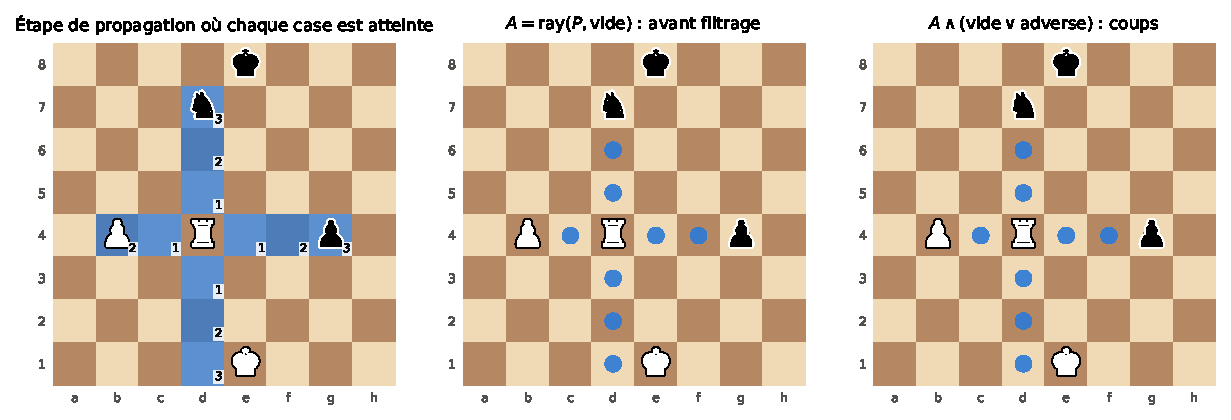
\includegraphics[width=\textwidth]{figs/glisseur.pdf}
\caption{Tour en d4. À gauche, le numéro de l'étape où le front atteint chaque case. Vers le haut,
le front s'arrête sur le cavalier noir d7, vers la gauche sur le pion blanc b4, vers la droite sur
le pion noir g4. Au milieu, le masque avant filtrage contient encore b4. À droite, le filtrage
retire b4, qui porte une pièce amie, et garde d7 et g4, qui sont des prises.}
\end{figure}

Chaque direction demande au plus 7 pas. Le fou suit les 4 diagonales, la tour les 4 directions
orthogonales, la dame les 8.

\subsection{Les pions, le roque et la prise en passant}
Les pions ne se déplacent pas comme ils prennent, mais leurs coups restent des décalages assortis
de conditions.
\begin{itemize}
\item Avance simple des blancs : $\shift(\text{pions}, -1, 0) \wedge \text{vide}$.
\item Avance double : depuis la rangée de départ, si les deux cases sont vides.
\item Prises : les deux décalages diagonaux, restreints aux pièces adverses et à la case de prise
en passant.
\end{itemize}
Le roque se vérifie en lisant quelques cases. Le roi et la tour doivent être à leur place, les
cases entre eux vides, les droits de roque intacts, et aucune case traversée par le roi ne doit
être attaquée.

\subsection{L'attaque et l'échec}
Le masque des cases attaquées par les blancs, $\mathrm{att}_{\text{blancs}}$, est l'union des
masques de toutes leurs pièces. Le roi noir est en échec si ce masque contient sa case. En
matrices, on fait un produit élément par élément, puis une somme :
\[ \text{échec} \iff \sum_{i,j} \bigl(\mathrm{att}_{\text{blancs}} \odot [B = -6]\bigr)_{ij} > 0. \]

\begin{exemple}{le coup du berger}
Après 1.e4 e5 2.Fc4 Cc6 3.Dh5 Cf6 4.Dxf7, le moteur calcule
\[ \sum_{i,j} (\mathrm{att} \odot [B=-6])_{ij} = 1,\qquad \text{cases de fuite} = 0,\qquad \texttt{status()} = \text{« checkmate »}
\unskip \]
Le roi est attaqué et aucun coup légal ne pare l'échec. Il est mat.
\end{exemple}

\begin{figure}[H]
\centering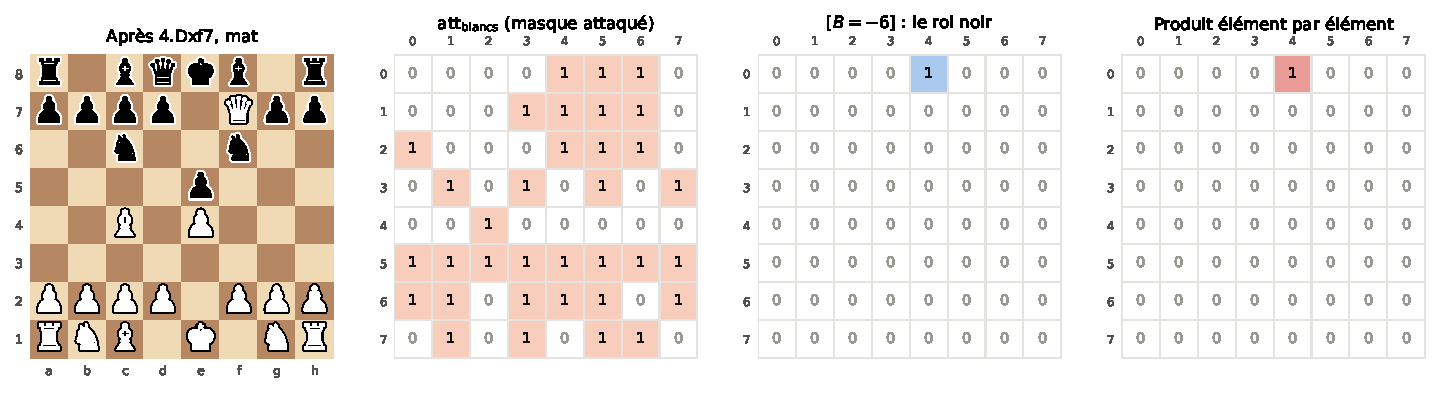
\includegraphics[width=\textwidth]{figs/echec.pdf}
\caption{Le test d'échec en trois matrices. Les cases attaquées, la case du roi, puis leur
produit, qui contient un seul 1, en e8.}
\end{figure}

\begin{retenir}
Toutes les règles de déplacement s'écrivent avec des décalages et des opérations logiques case
par case. Le moteur ne boucle pas sur les pièces et ne teste jamais les bords. La même formule
s'applique à un plateau seul ou à un lot de plateaux de forme $(N, 8, 8)$.
\end{retenir}

% =====================================================================================================
\section{Un coup est une matrice}

\subsection{Le coup simple : e2-e4}
Jouer e2-e4, c'est vider e2 et poser en e4 ce qui se trouvait en e2. Soit $f$ la case de départ,
$t$ la case d'arrivée, et $E_{ab}$ la matrice qui contient un seul 1, en ligne $a$ et colonne $b$.
Alors
\[ T = I - E_{ff} - E_{tt} + E_{tf},\qquad b' = T\,b. \]
\begin{itemize}
\item $-E_{ff}$ annule la ligne $f$, et la case de départ devient vide.
\item $-E_{tt}$ annule la ligne $t$, et le contenu de la case d'arrivée disparaît.
\item $+E_{tf}$ copie $b_f$ dans $b'_t$, et la pièce arrive.
\end{itemize}

\begin{figure}[H]
\centering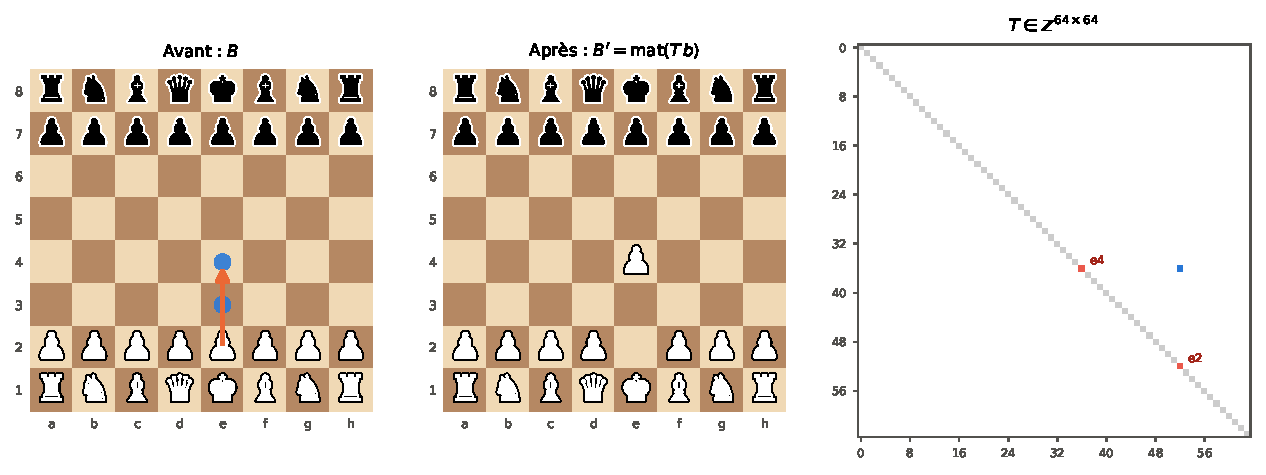
\includegraphics[width=\textwidth]{figs/coup_pion.pdf}
\caption{e2-e4. Les points bleus marquent les destinations du pion. La matrice $T$ est presque
l'identité (diagonale grise). Sa diagonale s'annule en e2 et en e4 (rouge), et un seul coefficient
se trouve hors de la diagonale (bleu), en ligne e4 et colonne e2.}
\end{figure}

Restreinte aux cases qui changent, la matrice tient en quelques lignes :
\[ S = (e4=36, e2=52),\quad T_S = \begin{pmatrix}0 & 1 \\ 0 & 0\end{pmatrix},\quad b_S = \begin{pmatrix}0 \\ 1\end{pmatrix}\;\longmapsto\; (Tb)_S = \begin{pmatrix}1 \\ 0\end{pmatrix} \]
\[ R_S = \begin{pmatrix}0 & 0 \\ 1 & 0\end{pmatrix},\qquad (R\,b')_S = \begin{pmatrix}0 \\ 1\end{pmatrix} \]
Ici, on retrouve exactement $b_S$. Rang de $T$ : 63 sur 64.
\unskip

La matrice $R$ défait le coup. Elle remet en $f$ ce qui se trouve en $t$. Le rang 63 signifie
qu'une dimension est perdue, celle du contenu de la case d'arrivée, ici une case vide.

\subsection{La prise : l'information détruite}
Une prise a la même matrice qu'un coup simple. Seul $b$ diffère, car la case $t$ n'était pas
vide. Le terme $-E_{tt}$ efface alors une pièce.
\begin{figure}[H]
\centering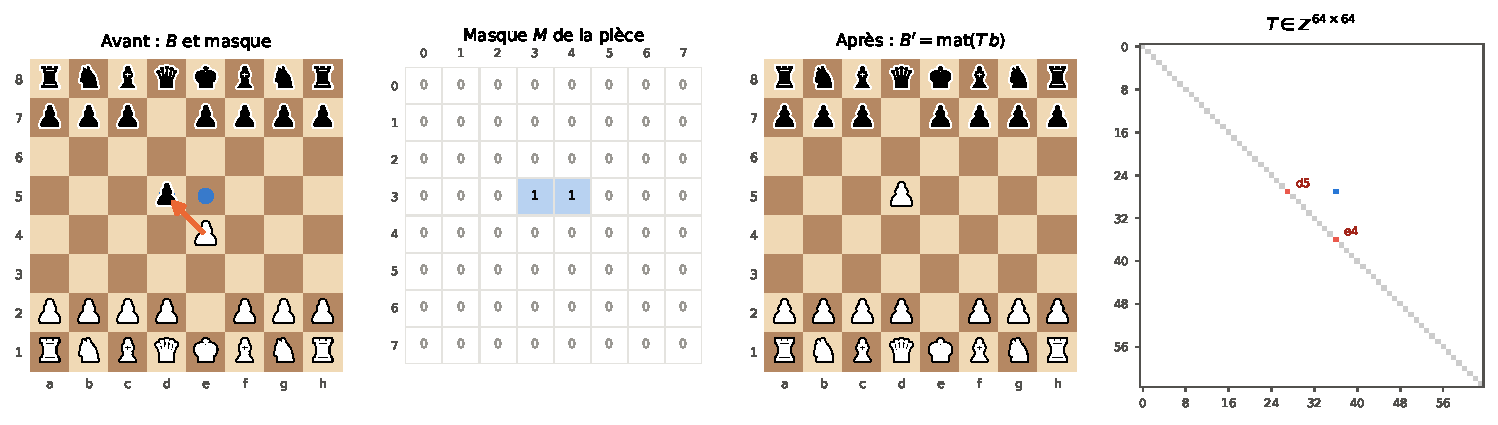
\includegraphics[width=\textwidth]{figs/coup_prise.pdf}
\caption{1.e4 d5 2.exd5. La matrice a la même forme que pour e2-e4. La ligne $t$ de $T$ efface le
pion noir de d5.}
\end{figure}
\[ S = (d5=27, e4=36),\quad T_S = \begin{pmatrix}0 & 1 \\ 0 & 0\end{pmatrix},\quad b_S = \begin{pmatrix}-1 \\ 1\end{pmatrix}\;\longmapsto\; (Tb)_S = \begin{pmatrix}1 \\ 0\end{pmatrix} \]
\[ R_S = \begin{pmatrix}0 & 0 \\ 1 & 0\end{pmatrix},\qquad (R\,b')_S = \begin{pmatrix}0 \\ 1\end{pmatrix} \]
Ici, la pièce prise n'est pas restituée : l'information est perdue. Rang de $T$ : 63 sur 64.
\unskip

Voilà pourquoi on ne peut pas inverser $T$. Elle est singulière, et la pièce prise appartient à
son noyau. Revenir en arrière demande une information que $T$ a effacée.

\subsection{La promotion : un coefficient}
Pour changer un pion en dame, on remplace le 1 de $E_{tf}$ par un coefficient $k$, ce qui donne
$T = I - E_{ff} - E_{tt} + k\,E_{tf}$. Le pion blanc vaut $+1$, donc la case d'arrivée reçoit
$k\cdot(+1) = +5$, une dame. Un pion noir donne $k\cdot(-1) = -5$. Le même coefficient sert aux
deux camps.
\begin{figure}[H]
\centering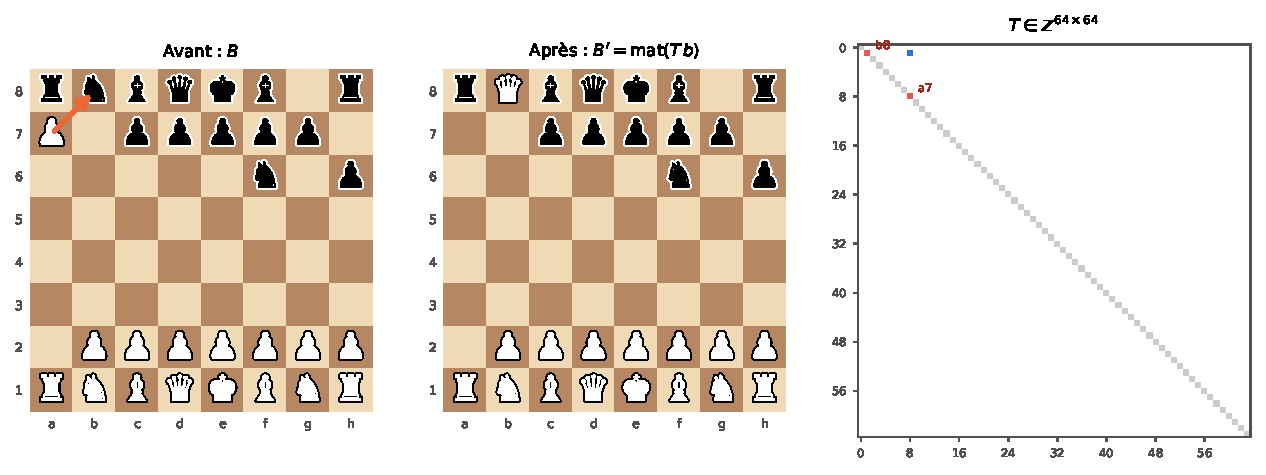
\includegraphics[width=\textwidth]{figs/coup_promotion.pdf}
\caption{a7xb8=D, une promotion avec prise. Le coefficient bleu vaut 5.}
\end{figure}
\[ S = (b8=1, a7=8),\quad T_S = \begin{pmatrix}0 & 5 \\ 0 & 0\end{pmatrix},\quad b_S = \begin{pmatrix}-2 \\ 1\end{pmatrix}\;\longmapsto\; (Tb)_S = \begin{pmatrix}5 \\ 0\end{pmatrix} \]
\[ R_S = \begin{pmatrix}0 & 0 \\ \tfrac{1}{5} & 0\end{pmatrix},\qquad (R\,b')_S = \begin{pmatrix}0 \\ 1\end{pmatrix} \]
Ici, $R$ ne rend pas la pièce prise, dont la valeur est perdue. La matrice $T$ est de rang 63 sur 64.
\unskip

Le retour divise par $k$. La matrice $R$ contient $\tfrac15$, qui change la dame en pion.

\subsection{La prise en passant : une case de plus}
Le pion qui prend en passant arrive sur une case vide, et le pion pris se trouve à côté. On ajoute
$-E_{cc}$ pour vider cette troisième case $c$, d'où
$T = I - E_{ff} - E_{tt} - E_{cc} + E_{tf}$.
\begin{figure}[H]
\centering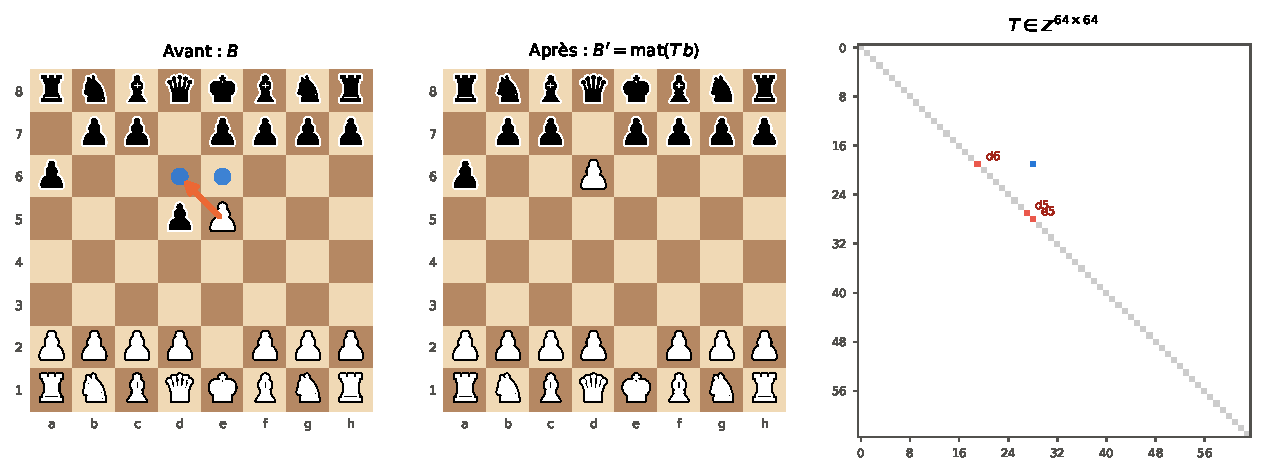
\includegraphics[width=\textwidth]{figs/coup_enpassant.pdf}
\caption{1.e4 a6 2.e5 d5 3.exd6 e.p. Trois cases changent. La case e5 se vide, d6 reçoit le pion
blanc et d5 perd le pion noir.}
\end{figure}
\[ S = (d6=19, d5=27, e5=28),\quad T_S = \begin{pmatrix}0 & 0 & 1 \\ 0 & 0 & 0 \\ 0 & 0 & 0\end{pmatrix},\quad b_S = \begin{pmatrix}0 \\ -1 \\ 1\end{pmatrix}\;\longmapsto\; (Tb)_S = \begin{pmatrix}1 \\ 0 \\ 0\end{pmatrix} \]
\[ R_S = \begin{pmatrix}0 & 0 & 0 \\ 0 & 1 & 0 \\ 1 & 0 & 0\end{pmatrix},\qquad (R\,b')_S = \begin{pmatrix}0 \\ 0 \\ 1\end{pmatrix} \]
Ici, $R$ ne rend pas la pièce prise, dont la valeur est perdue. La matrice $T$ est de rang 62 sur 64.
\unskip

\subsection{Le roque : deux déplacements dans une matrice}
Le roque déplace le roi et la tour. On superpose deux coups simples dans la même matrice :
\[ T = I - E_{ff} - E_{tt} + E_{tf} - E_{f'f'} - E_{t't'} + E_{t'f'}. \]
\begin{figure}[H]
\centering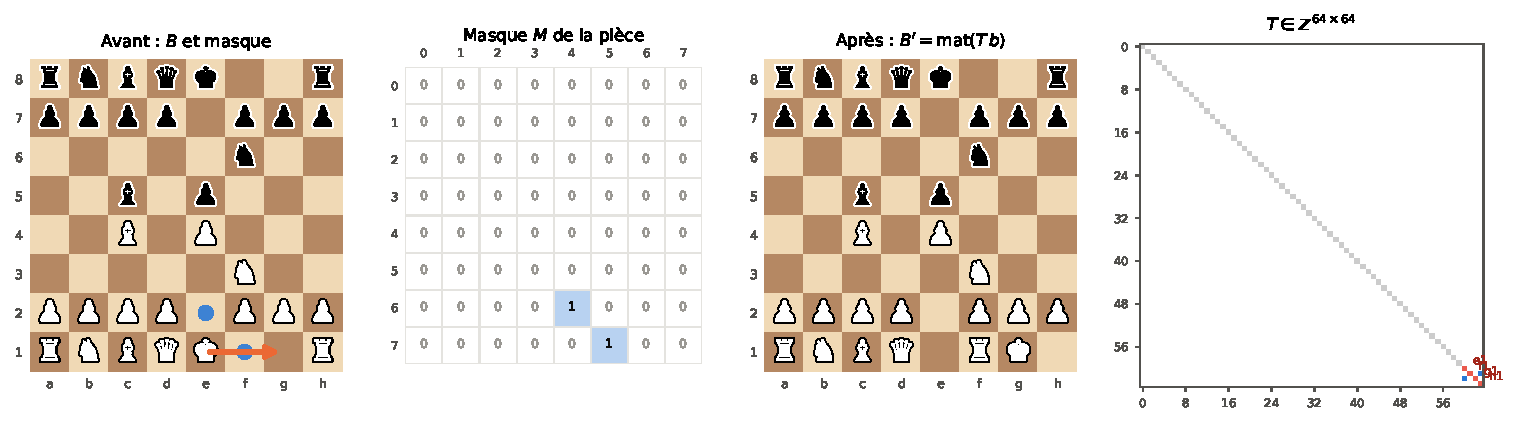
\includegraphics[width=\textwidth]{figs/coup_roque.pdf}
\caption{Petit roque blanc, roi e1-g1 et tour h1-f1. La matrice a deux coefficients hors de la
diagonale.}
\end{figure}
\[ S = (e1=60, f1=61, g1=62, h1=63),\quad T_S = \begin{pmatrix}0 & 0 & 0 & 0 \\ 0 & 0 & 0 & 1 \\ 1 & 0 & 0 & 0 \\ 0 & 0 & 0 & 0\end{pmatrix},\quad b_S = \begin{pmatrix}6 \\ 0 \\ 0 \\ 4\end{pmatrix}\;\longmapsto\; (Tb)_S =\begin{pmatrix}0 \\ 4 \\ 6 \\ 0\end{pmatrix} \]
\[ R_S = \begin{pmatrix}0 & 0 & 1 & 0 \\ 0 & 0 & 0 & 0 \\ 0 & 0 & 0 & 0 \\ 0 & 1 & 0 & 0\end{pmatrix},\qquad (R\,b')_S = \begin{pmatrix}6 \\ 0 \\ 0 \\ 4\end{pmatrix} \]
\begin{itemize}
\item \textbf{Coups de la pièce.} Le masque $M$ contient 2 destinations, et la pièce a 3 coups légaux dans cette position.
\item \textbf{Matrice.} Ici, $R$ rend $b_S$ sans perte. La matrice $T$ est de rang 62 sur 64.
\item \textbf{Forme réduite.} La ligne $(f, t, k, c, f', t') = (60, 62, 1, 64, 63, 61)$ donne les 4 écritures $b'_{62} = b_{60},\ b'_{60} = 0,\ b'_{61} = b_{63},\ b'_{63} = 0$.
\item \textbf{Plan.} Le coup appartient au plan $p = 68$ (« O-O »), de décalage $\delta_p = +2$, et $t = f + \delta_p = 60 +2 = 62$.
\end{itemize}
\unskip

\subsection{Une partie est un produit de matrices}
Jouer $n$ coups revient à multiplier $n$ matrices, $b_n = T_n \cdots T_1\, b_0 = G\, b_0$. La
matrice $G$ résume la partie entière. Chacune de ses lignes contient au plus un coefficient non
nul, et deux lignes n'en ont jamais dans la même colonne. On appelle une telle matrice une
\emph{permutation partielle pondérée}. Elle se stocke dans deux plateaux d'étiquettes. Pour chaque
case $i$, $\mathrm{src}_i$ indique de quelle case initiale vient son contenu, et
$\mathrm{coef}_i$ le facteur qui le multiplie, soit 0 si la case a été vidée et $k$ après une
promotion. On a alors $b_n[i] = \mathrm{coef}_i\cdot b_0[\mathrm{src}_i]$, sans aucune matrice
$64\times64$.

\begin{exemple}{la partie espagnole, variante d'échange}
1.e4 e5 2.Cf3 Cc6 3.Fb5 a6 4.Fxc6 dxc6. Le produit des huit matrices donne $G$.
$G$ est de rang 56 sur 64. Ses lignes nulles sont les cases vidées (b8, a7, d7, e7, b5, e2, f1, g1). Parmi ses colonnes nulles, 2 portaient une pièce au départ, b8 et f1, les deux pièces prises.
\unskip
\end{exemple}

\begin{figure}[H]
\centering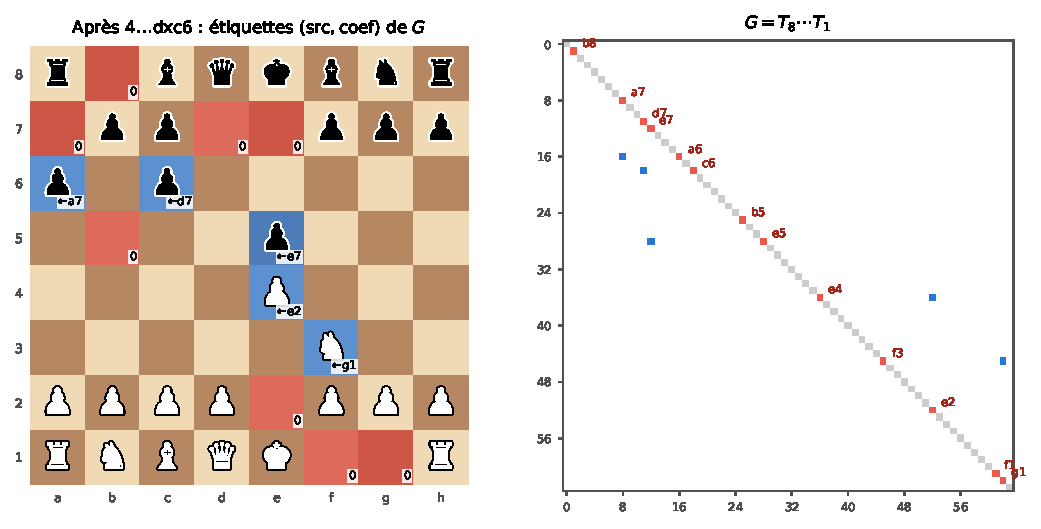
\includegraphics[width=\textwidth]{figs/composition.pdf}
\caption{À gauche, l'étiquette de chaque case. En e4, « ←e2 » signifie que le contenu de e4 vient
de la case initiale e2. « 0 » marque une case vidée. En c6, l'étiquette « ←d7 » indique que le pion
a pris le fou, lui-même venu de f1. La colonne f1 de $G$ est donc nulle, et plus aucune ligne de
$G$ ne transporte le fou.}
\end{figure}

Le rang de $G$ est le nombre de ses lignes non nulles, et chaque case vidée en retire une. Parmi
les colonnes nulles, celles qui portaient une pièce au départ correspondent aux pièces prises.

\subsection{Revenir en arrière : trois réponses}
Un coup sans prise s'inverse sans difficulté, car $R\,T\,b = b$. Avec une prise, $T$ n'est pas
inversible. Le projet a exploré trois façons de traiter ce cas.

\paragraph{1. L'inverse affine, avec une pile des prises.} On conserve à part la liste des pièces
prises. Le retour s'écrit $b = R\,b' + \text{correction}$, où la correction remet la pièce prise
sur sa case. Les fonctions \code{reverse\_matrix} et \code{invert\_game} procèdent ainsi.

\paragraph{2. L'espace étendu avec un cimetière.} On ajoute au vecteur 30 cases, une par pièce
capturable, ce qui donne $x\in\mathbb{Z}^{94}$. Une prise devient alors un cycle de trois cases. La
pièce qui prend va en $t$, la pièce prise va au cimetière, et la case de départ reçoit le vide qui
occupait le cimetière. Chaque coup devient une matrice \emph{monomiale}, qui a un seul coefficient
non nul par ligne et par colonne. Une telle matrice est inversible.
\[ \tilde T_S = \begin{pmatrix}0 & 0 & 1 \\ 1 & 0 & 0 \\ 0 & 1 & 0\end{pmatrix},\quad x_S = \begin{pmatrix}1 \\ -1 \\ 0\end{pmatrix}\;\longmapsto\; (\tilde T x)_S = \begin{pmatrix}0 \\ 1 \\ -1\end{pmatrix},\quad \det \tilde T = +1,\quad \tilde T^{-1} = \tilde T^{\top}
\unskip \]
\begin{figure}[H]
\centering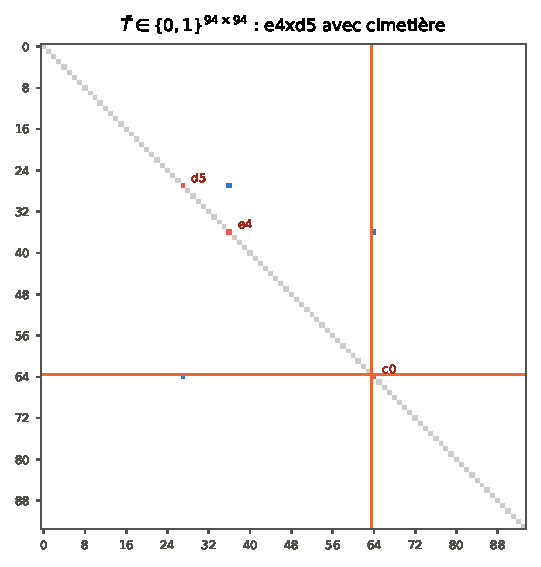
\includegraphics[width=.55\textwidth]{figs/cimetiere.pdf}
\caption{La prise e4xd5 dans l'espace à 94 dimensions. Les lignes orange séparent le plateau (64
cases) du cimetière (30 cases). La pièce prise n'est plus effacée, elle est rangée en c0.}
\end{figure}
Sur toute une partie, $\tilde G = \tilde T_n\cdots\tilde T_1$ reste monomiale, et une seule
multiplication par $\tilde G^{-1}$ ramène l'état final à la position de départ. Le script
\code{invert\_full\_game.py} le vérifie sur une partie complète.

\paragraph{3. Sans cimetière, une relation.} Si l'on ne conserve rien, l'inverse d'un coup n'est
plus une fonction mais une \emph{relation} :
\[ b_{\text{prev}} = R\,b + c\,e_t,\qquad c\in\{0\}\cup\{\text{pièces adverses restaurables}\}. \]
Le paramètre libre $c$ représente l'information détruite par la prise. En marche arrière, chaque
valeur possible de $c$ ouvre une branche.

\begin{figure}[H]
\centering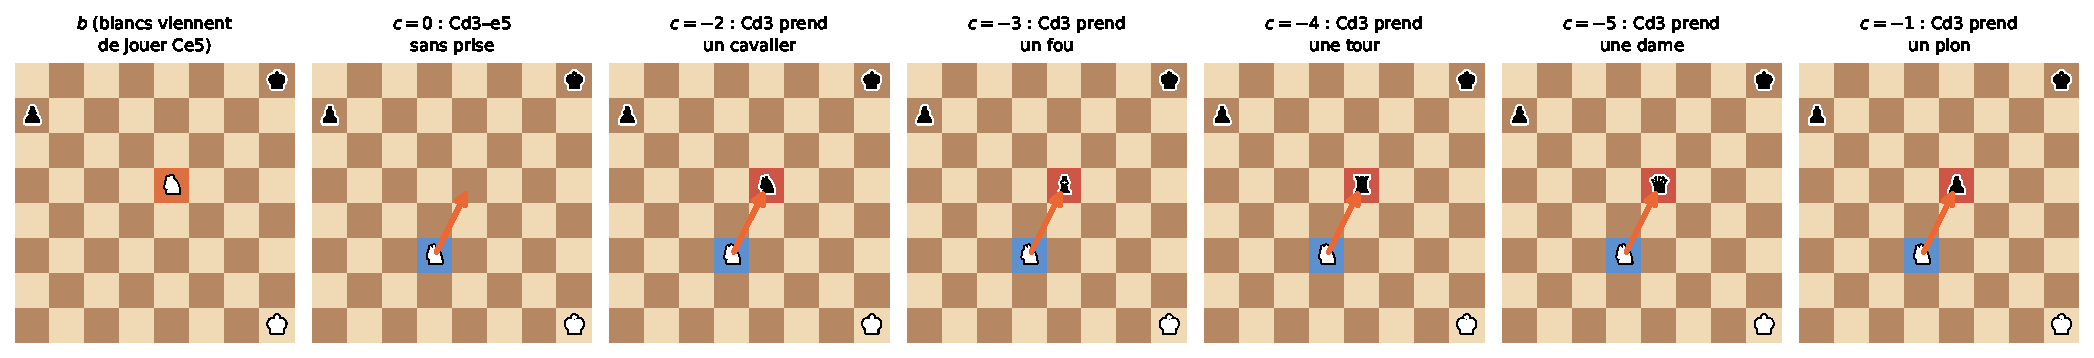
\includegraphics[width=\textwidth]{figs/retro.pdf}
\caption{Les blancs viennent de jouer un cavalier en e5. S'il venait de d3, il a pu ne rien
prendre, ou prendre une pièce noire de l'une des cinq sortes. Chaque valeur de $c$ donne un
prédécesseur différent, et tous sont légaux.}
\end{figure}
\noindent Pour cette position, 51 prédécesseurs légaux à un demi-coup, depuis 9 cases d'origine (c4, c6, d3, d7, f3, g1, g2, g4, h2) ; 6 d'entre eux partent de d3.
\unskip

\subsection{Imposer une fin : le mat étouffé}
La relation arrière permet de retourner la question. Au lieu de chercher le meilleur coup, on fixe
une condition finale et on cherche une suite de coups qui y conduit. Le module \code{impose.py}
procède en deux temps.
\begin{enumerate}
\item \textbf{Synthèse des buts.} Le programme ne reçoit aucune position finale. Il en fabrique
en modifiant légèrement le plateau autour du roi visé, sans ajouter de pièce, et garde celles qui
satisfont le prédicat. Pour le mat étouffé, le prédicat exige un échec donné par un cavalier et un
roi entouré de ses propres pièces.
\item \textbf{Reliaison par rencontre au milieu.} Le programme développe les coups légaux depuis
la position actuelle. Depuis chaque but, il remonte d'un demi-coup grâce à la relation
$b_{\text{prev}} = R\,b + c\,e_t$. Une position atteinte des deux côtés fournit la suite de
coups.
\end{enumerate}

\begin{exemple}{le mat de Philidor, redécouvert}
On part de la position de gauche, avec pour seule consigne « mat étouffé » en 3 demi-coups au
plus. Le moteur trouve \texttt{e6f6}, \texttt{f8g8}, \texttt{h6f7}
\unskip. La dame menace g7, la tour noire vient la
défendre en g8, et le cavalier donne mat en f7.
\end{exemple}
\begin{figure}[H]
\centering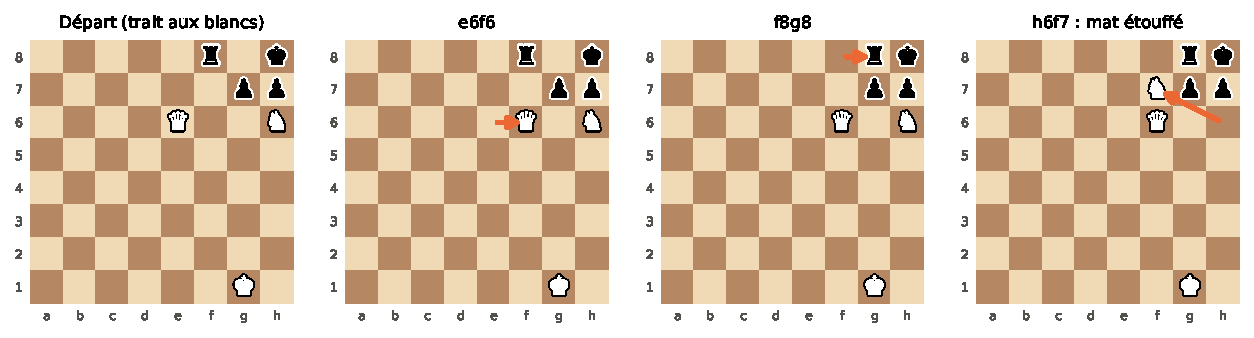
\includegraphics[width=\textwidth]{figs/etouffe.pdf}
\caption{La suite trouvée par \code{impose(position, is\_smothered\_mate)}. Personne n'a fourni la
position finale. Le programme l'a construite, puis reliée à la position de départ.}
\end{figure}

\begin{retenir}
Un coup s'écrit $T = I - E_{ff} - E_{tt} + k\,E_{tf}$, avec un terme de plus pour la prise en
passant et un second déplacement pour le roque. Une partie est un produit de telles matrices, qui
tient dans deux plateaux d'étiquettes. Une prise détruit de l'information. Si on la range dans un
cimetière, toutes les matrices deviennent inversibles. Sinon, elle réapparaît en marche arrière
sous forme de branches, ce qui permet d'imposer une condition finale.
\end{retenir}

% =====================================================================================================
\section{Des millions de positions à la fois : le GPU}

Une carte graphique applique la même opération à des millions de données en parallèle. Les
parties précédentes ont tout écrit en décalages et en opérations case par case. Il reste à empiler
les positions.

\subsection{Empiler les plateaux}
On range $N$ plateaux dans un tableau de forme $(N, 65)$. La 65\textsuperscript{e} colonne,
\code{NONE}, est une sentinelle qui vaut toujours zéro. Elle joue le rôle d'une case inexistante.
Un coup sans prise en passant vide la case \code{NONE}, ce qui ne change rien, et aucun coup ne
demande donc de traitement particulier. Un coup est une ligne de six entiers $(f, t, k, c, f',
t')$ :
\[ \texttt{coups} = \begin{pmatrix}52 & 36 & 1 & 64 & 64 & 64 \\ 51 & 35 & 1 & 64 & 64 & 64 \\ 62 & 45 & 1 & 64 & 64 & 64 \\ 57 & 42 & 1 & 64 & 64 & 64\end{pmatrix}
\unskip \]
Appliquer $T$ à chaque plateau revient alors à une lecture groupée (\emph{gather}) suivie d'une
écriture groupée (\emph{scatter}). Le GPU calcule \code{out[t] = k·b[f]}, puis \code{out[f] = 0} et
\code{out[c] = 0}, et fait de même pour la tour du roque. La matrice $64\times64$ n'est jamais
construite.

\begin{figure}[H]
\centering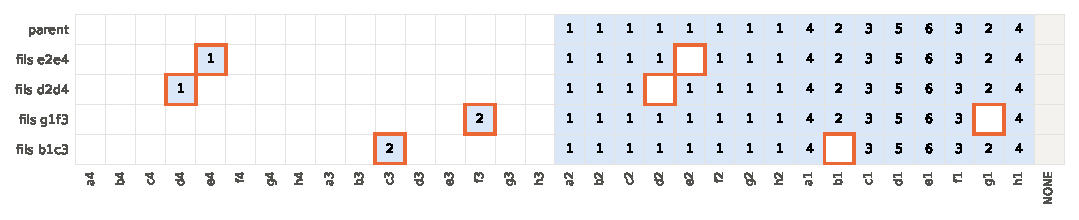
\includegraphics[width=\textwidth]{figs/lots.pdf}
\caption{Un parent et quatre fils, vus comme des lignes d'un tableau (cases a4 à h1, puis la
sentinelle). Deux cellules seulement changent dans chaque fils (encadrés orange).}
\end{figure}

\subsection{Les 70 plans de coups}
Pour générer tous les coups d'un lot, on construit un masque de forme $(N, 70, 64)$. Chaque plan
$p$ correspond à un décalage fixe $\delta_p$. Dans ce plan, la case $f$ vaut vrai si la pièce posée
en $f$ peut jouer ce décalage. Les 70 plans couvrent tous les coups possibles :
\begin{itemize}
\item 56 plans de rayons, soit 8 directions et 7 distances, pour la dame, la tour, le fou et le roi
(distance 1) ;
\item 8 plans de sauts de cavalier ;
\item 4 plans de pions, pour l'avance simple, l'avance double et les deux prises ;
\item 2 plans de roque.
\end{itemize}

\begin{figure}[H]
\centering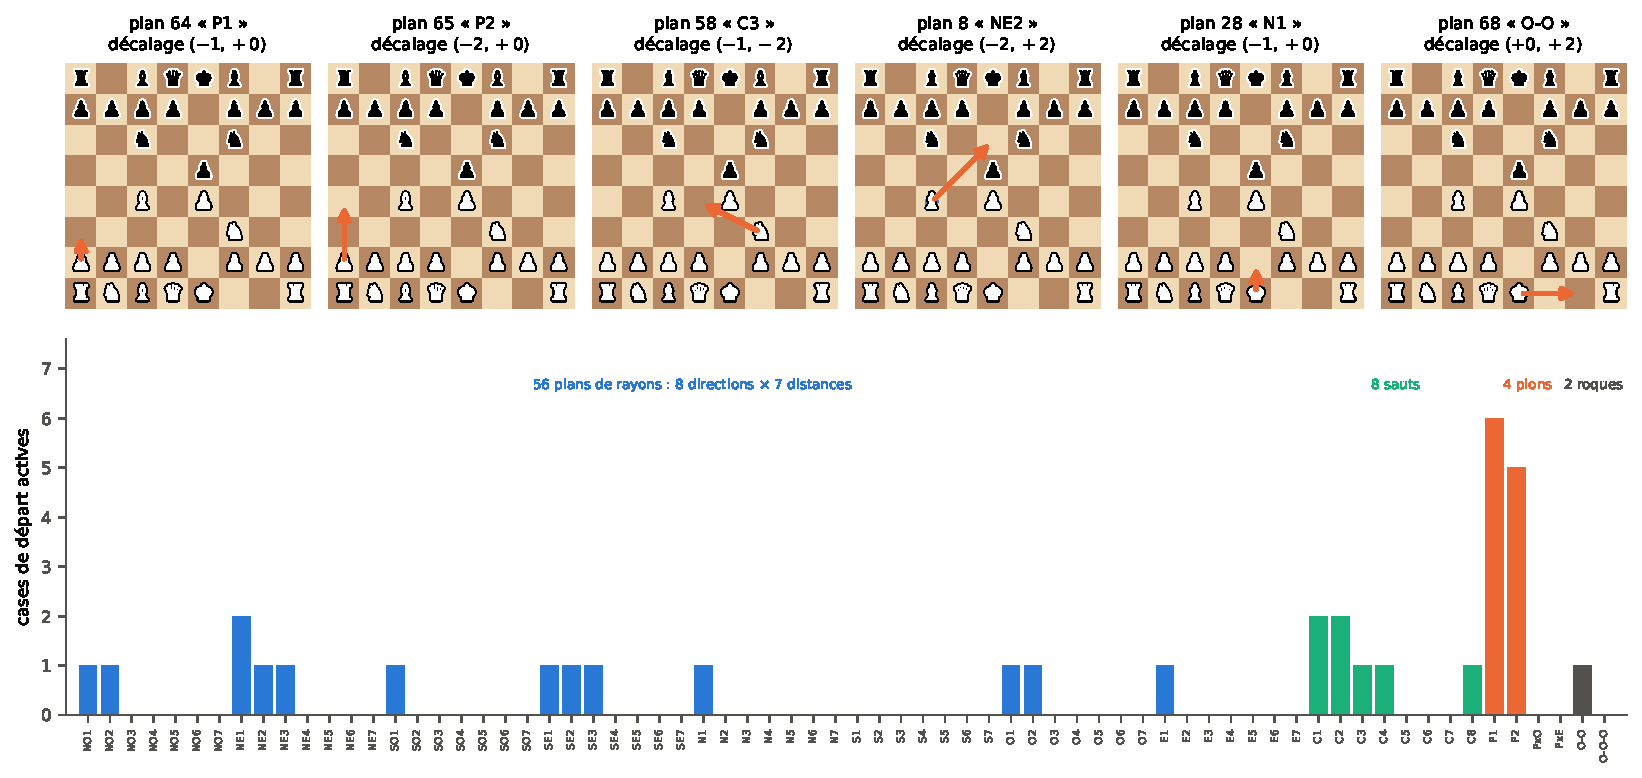
\includegraphics[width=\textwidth]{figs/plans.pdf}
\caption{Après 1.e4 e5 2.Cf3 Cc6 3.Fc4 Cf6. En haut, six plans, où les points marquent les cases de
départ et la flèche montre un coup du plan. En bas, le nombre de cases de départ actives dans
chacun des 70 plans.}
\end{figure}

Le décodage tient en une opération. La liste des indices non nuls du masque donne des couples
(plan, case de départ), et la case d'arrivée vaut $t = f + \delta_p$.
\begin{center}\small\begin{tabular}{rlrlrl}\toprule plan $p$ & nom & départ $f$ & case & $t = f + \delta_p$ & coup\\\midrule
0 & NO1 & 34 & c4 & 25 & \texttt{c4b5}\\
14 & SO1 & 34 & c4 & 41 & \texttt{c4b3}\\
43 & O2 & 63 & h1 & 61 & \texttt{h1f1}\\
58 & C3 & 45 & f3 & 35 & \texttt{f3d4}\\
64 & P1 & 51 & d2 & 43 & \texttt{d2d3}\\\bottomrule\end{tabular}
\unskip\end{center}
Dans cette position, le masque contient 33 coups pseudo-légaux, tous légaux
\unskip. Sur des centaines de
positions tirées au hasard, les coups obtenus sont identiques à ceux de \code{python-chess}.

\subsection{Le test d'échec vu depuis le roi}
Un coup pseudo-légal est légal si notre roi n'est pas en échec après le coup. Calculer les masques
d'attaque de tout le camp adverse coûterait cher. On regarde plutôt depuis le roi. On lit les cases
de ses rayons, de ses sauts de cavalier et de son voisinage, ainsi que les deux cases d'où un pion
pourrait l'attaquer. Si la première pièce rencontrée sur un rayon orthogonal est une dame ou une
tour adverse, ou sur une diagonale une dame ou un fou adverse, le roi est en échec.
\begin{figure}[H]
\centering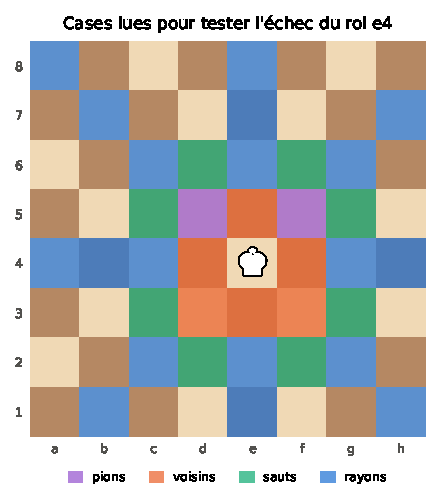
\includegraphics[width=.42\textwidth]{figs/vue_roi.pdf}
\caption{Les cases lues pour un roi en e4. Les tables d'indices sont calculées une fois pour
toutes, et les indices hors du plateau pointent sur la sentinelle.}
\end{figure}
\noindent 56 indices de rayons (27 sur le plateau), 8 sauts de cavalier (8), 8 voisins (8), 2 pions (2) : 74 lectures par plateau.
\unskip{} Le GPU les effectue en une seule lecture groupée pour tout
le lot.

\subsection{Bitboards et noyau fusionné}
Le dernier gain vient d'un noyau CUDA écrit à la main. Ce noyau représente chaque masque par un
entier de 64 bits, où le bit $i$ correspond à la case $i$. Un décalage de masque devient un
décalage de bits :
\[ \texttt{pions} = \texttt{0x00FF000000000000},\qquad (\texttt{pions} \gg 8)\ \&\ \lnot\,\texttt{occ} = \texttt{0x0000FF0000000000}
\unskip \]
Chaque fil d'exécution traite un parent. Il compte d'abord ses fils. Une somme préfixe attribue
ensuite à chaque parent sa place dans le tableau de sortie, puis chaque fil écrit ses enfants. Le
noyau produit les mêmes enfants, dans le même ordre, que la version \code{torch}, environ dix fois
plus vite.

\subsection{Le débit obtenu}
Le \emph{perft} compte toutes les positions atteignables à une profondeur donnée. C'est le test de
référence d'un générateur de coups, car les valeurs exactes sont connues et la moindre erreur les
modifie.
\begin{figure}[H]
\centering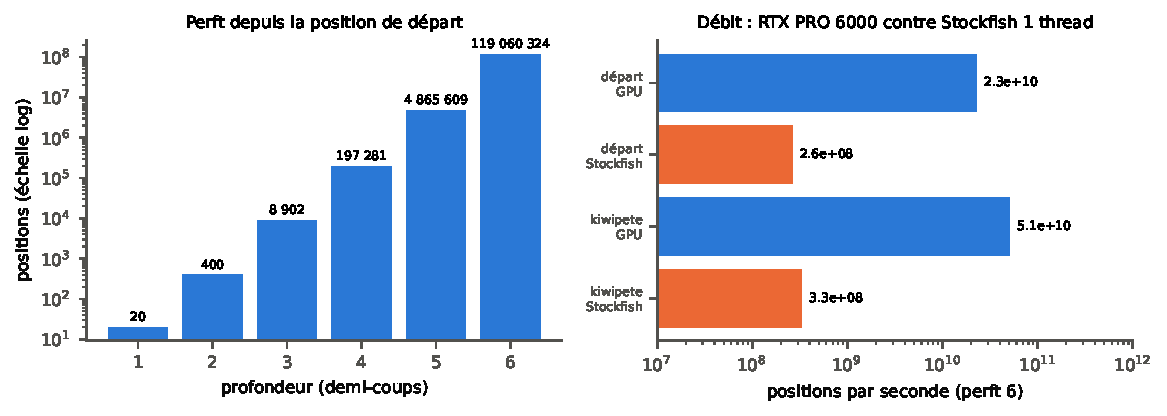
\includegraphics[width=\textwidth]{figs/perft.pdf}
\caption{À gauche, la croissance du nombre de positions, de 20 à 119 millions en 6 demi-coups. Le
script recalcule les profondeurs 1 à 5 sur CPU. À droite, le débit d'une RTX PRO 6000 comparé à la
commande \code{go perft} de Stockfish.}
\end{figure}
Kiwipete est une position de test où chaque camp dispose de nombreux coups. Sur cette position, le
GPU compte les positions 157
\unskip~fois plus vite que Stockfish sur un cœur.

\begin{retenir}
Les plateaux s'empilent dans un tableau $(N, 65)$. Un coup est une ligne de six entiers, appliquée
par une lecture et une écriture groupées. Les 70 plans produisent en une passe tous les coups d'un
lot. Le GPU atteint $5\times10^{10}$ positions par seconde en perft.
\end{retenir}

% =====================================================================================================
\section{Chercher le meilleur coup}

Générer vite ne suffit pas. Pour choisir un coup, il faut comparer des suites de coups. Cette partie
part d'un arbre jouet à 9 feuilles et construit pas à pas l'alpha-bêta par lots du moteur.

\subsection{Minimax et negamax}
Les blancs choisissent le coup qui maximise l'évaluation, les noirs celui qui la minimise. Dans
l'arbre jouet, la racine a trois fils, et chaque fils a trois feuilles évaluées. Un fils vaut le
minimum de ses feuilles, et la racine vaut le maximum de ses fils.

Le moteur utilise la forme \emph{negamax}, qui traite les deux camps de la même façon. Chaque nœud
évalue la position du point de vue du camp au trait, et
\[ v(p) = \max_{c\,\in\,\text{fils}(p)} \bigl(-v(c)\bigr). \]

\subsection{L'écriture (max, +)}
Remplaçons l'addition par le maximum, et la multiplication par l'addition. On obtient le
semi-anneau $(\max, +)$, dans lequel le produit d'une matrice par un vecteur s'écrit
$(A\otimes x)_i = \max_j (A_{ij} + x_j)$. Posons $A_{ij}=0$ si $j$ est un fils de $i$, et
$A_{ij}=-\infty$ sinon. Un niveau de negamax devient alors un produit matrice-vecteur :
\[ A_1 = \begin{pmatrix}0 & 0 & 0 & -\infty & -\infty & -\infty & -\infty & -\infty & -\infty \\ -\infty & -\infty & -\infty & 0 & 0 & 0 & -\infty & -\infty & -\infty \\ -\infty & -\infty & -\infty & -\infty & -\infty & -\infty & 0 & 0 & 0\end{pmatrix}
 \]
\[ \begin{gathered}(-\ell)^{\top} = (-3, -12, -8, -2, -4, -6, -14, -5, -2) \\ v_1 = A_1 \otimes (-\ell) = (-3, -2, -2)^{\top},\quad v_0 = A_0 \otimes (-v_1) = 3
\unskip\end{gathered} \]
La recherche pleine largeur sur GPU procède ainsi, niveau par niveau. Elle forme un lot de parents,
puis un lot de fils, et prend un maximum par groupe de frères. Le calcul est simple et entièrement
parallèle. Sa limite est la taille de l'arbre.

\subsection{Pourquoi la pleine largeur ne suffit pas}
Une position d'échecs offre environ 35 coups. À $d$ demi-coups, l'arbre compte de l'ordre de
$35^d$ feuilles. Même à $2,5\times10^8$ nœuds par seconde, la pleine largeur plafonne à 4 à 6
demi-coups en quelques secondes, alors que Stockfish dépasse 20.

\begin{figure}[H]
\centering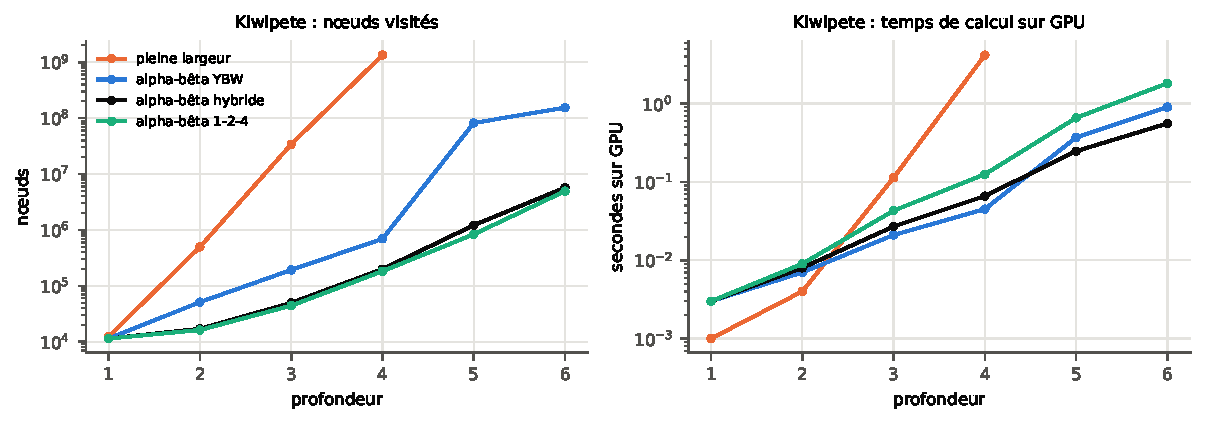
\includegraphics[width=\textwidth]{figs/exp_noeuds.pdf}
\caption{Kiwipete, mesures de l'incrément 1. À gauche, la pleine largeur visite un milliard de
nœuds en profondeur 4, l'alpha-bêta quelques centaines de milliers. À droite, le temps de calcul.
Sur GPU, visiter moins de nœuds n'accélère pas toujours la recherche, car des lots trop petits
laissent la carte sous-employée.}
\end{figure}

\subsection{L'alpha-bêta : ne pas lire ce qui ne change rien}
Parcourons l'arbre jouet de gauche à droite. Le premier fils vaut 3, donc les blancs sont sûrs
d'obtenir au moins 3. Dans le deuxième fils, la première feuille vaut 2. Comme les noirs y
choisiront le minimum, ce fils vaudra au plus 2. Il ne peut pas dépasser 3, et ses deux autres
feuilles ne servent à rien. C'est ce qu'on appelle une \emph{coupure}.

\begin{figure}[H]
\centering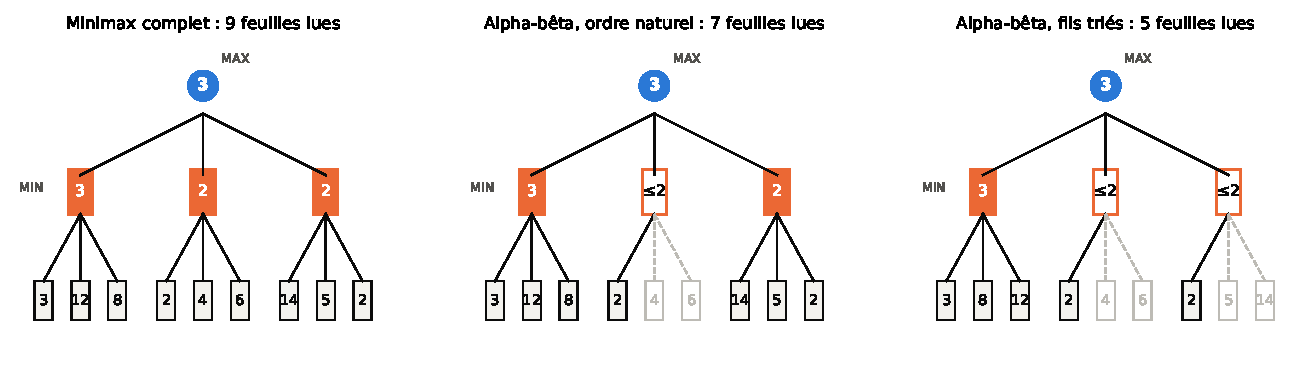
\includegraphics[width=\textwidth]{figs/arbre.pdf}
\caption{Le même arbre, parcouru de trois façons. Le minimax lit 9 feuilles. L'alpha-bêta en lit 7,
car il coupe le deuxième fils après sa première feuille. Si les feuilles sont triées de la
meilleure à la pire pour le camp qui choisit, il n'en lit que 5. La notation « $\le 2$ » désigne
une valeur connue seulement par une borne.}
\end{figure}

Formellement, chaque nœud reçoit une fenêtre $(\alpha, \beta)$. La borne $\alpha$ est ce que le
camp au trait s'est déjà assuré ailleurs, $\beta$ ce que l'adversaire s'est déjà assuré. Dès qu'un
fils atteint une valeur $\ge \beta$, les fils suivants ne servent plus. L'ordre des fils décide
donc du nombre de coupures. Dans le meilleur cas, avec $b$ coups par position et une profondeur
$d$, l'alpha-bêta lit $b^{\lceil d/2\rceil} + b^{\lfloor d/2\rfloor} - 1$ feuilles au lieu de
$b^d$. À temps égal, la profondeur atteignable double presque.

\subsection{L'alpha-bêta comme convergence d'intervalles}
Cette formulation relie l'alpha-bêta au calcul matriciel. Au lieu de calculer la valeur exacte de
chaque nœud, on tient à jour un intervalle $[L, U]$ qui la contient. Au départ, on sait seulement
que l'évaluation est bornée, ici par $[0, 15]$ dans l'arbre jouet. Chaque feuille lue resserre les
intervalles de ses ancêtres. Le calcul reprend les produits $(\max,+)$, appliqués d'un côté aux
bornes basses et de l'autre aux bornes hautes.
\begin{itemize}
\item \textbf{La convergence est monotone et finie.} Les intervalles ne peuvent que rétrécir, et
l'arbre est fini. Il ne s'agit pas d'une contraction au sens de Banach, qui garantirait une
vitesse géométrique. C'est une itération de Kleene, qui atteint son point fixe en un nombre fini
de pas.
\item \textbf{Le critère de décision se lit à la racine.} On peut jouer le coup $a$ dès que
$L(a) \ge \max_{b \ne a} U(b)$, car aucun autre coup ne peut plus le dépasser. Les valeurs exactes
des autres coups sont alors inutiles.
\end{itemize}

\begin{figure}[H]
\centering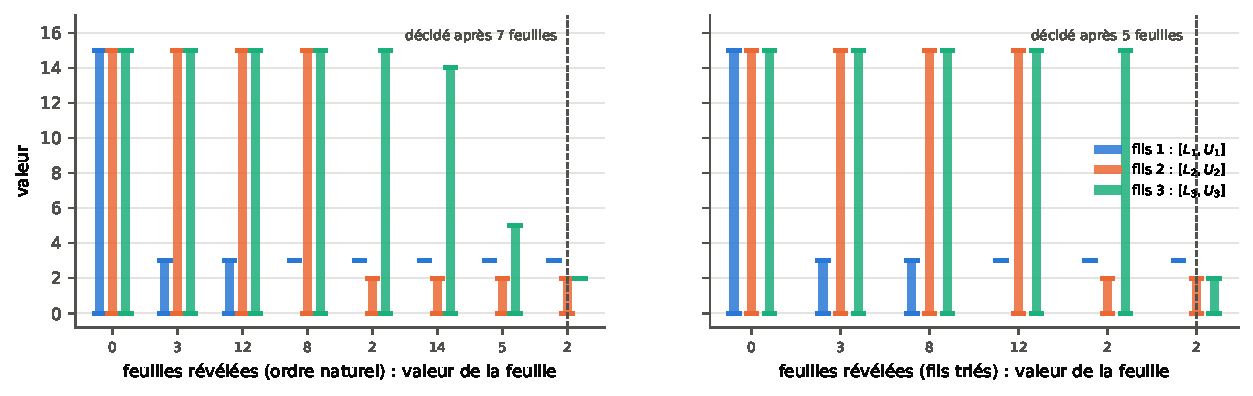
\includegraphics[width=\textwidth]{figs/intervalles.pdf}
\caption{Les intervalles des trois fils de la racine, feuille après feuille, dans l'ordre de
lecture de l'alpha-bêta. Le critère $L_1 \ge \max(U_2, U_3)$ devient vrai au moment où
l'alpha-bêta s'arrête.}
\end{figure}

Le critère est atteint après 7 feuilles dans l'ordre naturel, 5 avec les fils triés
\unskip, c'est-à-dire après autant de feuilles
que l'alpha-bêta en lit. L'alpha-bêta est donc la règle d'arrêt de cette convergence
d'intervalles. Cette lecture permet de le paralléliser. On peut lire les feuilles par paquets,
tant que le critère n'est pas atteint.

\subsection{L'alpha-bêta par lots : les vagues}
Sur GPU, lire les fils un par un donnerait des lots trop petits, et la plupart des cœurs
resteraient inactifs. On trie donc les fils du plus prometteur au moins prometteur, puis on les
découpe en \emph{vagues}. Le GPU évalue la première vague pour tous les parents du lot en même
temps. Les parents coupés quittent le lot. Les autres passent à la vague suivante, avec une
fenêtre plus étroite.

\begin{figure}[H]
\centering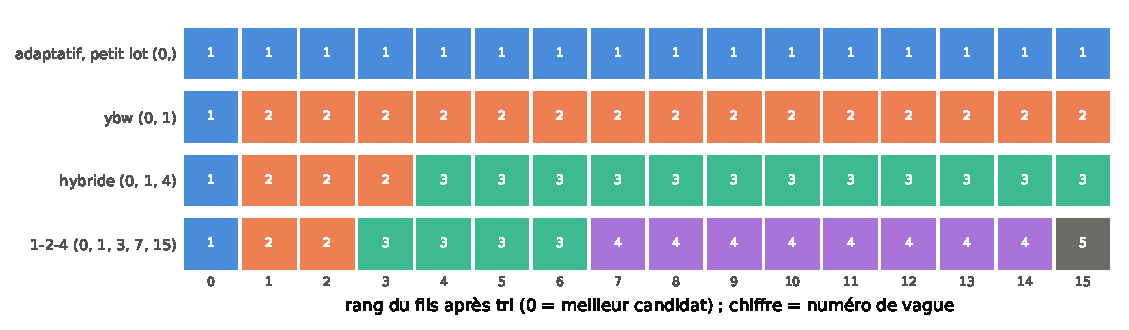
\includegraphics[width=.9\textwidth]{figs/vagues.pdf}
\caption{Découpage en vagues selon le rang du fils. YBW (\emph{Young Brothers Wait}) cherche
l'aîné seul, puis tous ses frères ensemble. Le mode hybride ajoute une vague intermédiaire. Le mode
1-2-4 double la taille de la vague à chaque étape. Le mode adaptatif choisit le découpage lot par
lot, selon la taille estimée du sous-arbre. Il prend tous les fils d'un coup sous $3\times10^4$
nœuds, YBW sous $3\times10^7$, hybride sous $3\times10^9$, et 1-2-4 au-delà.}
\end{figure}

Le tri des fils détermine l'efficacité de la première vague. Le tri MVV/LVA (\emph{Most Valuable
Victim, Least Valuable Attacker}) place les prises en tête, de la plus grosse victime prise par le
plus petit attaquant à l'inverse. Il coûte une lecture de table par fils. Pour chaque variante, un
test vérifie que le score est identique à celui de la pleine largeur. L'élagage ne change donc
jamais le résultat.

\subsection{Deux pièges rencontrés}
\paragraph{Le choix du coup à la racine.} En \emph{fail-soft}, un coup réfuté renvoie une borne
haute au lieu de sa vraie valeur. Cette borne pouvait égaler le score du meilleur coup, et
\code{argmax} choisissait alors parfois le coup réfuté. Le moteur a perdu ses 4 parties avant que
le bogue soit trouvé. La correction place la borne strictement sous le meilleur score. Un test
vérifie désormais que le coup joué, et pas seulement le score, vaut le minimax exact.

\paragraph{La pendule.} On ne peut pas prévoir le temps que prendra une profondeur de plus. Le
moteur cherche donc les coups de la racine par groupes de 1, 1, 2, 4 puis 8. Si le temps manque,
il joue le meilleur coup parmi les groupes terminés. Ce résultat est partiel, mais sûr. Un plafond
arrête tout à 1,5 fois le budget. Enfin, un coup de la racine qui répète une position déjà vue vaut
0, pour que le moteur ne laisse pas filer par répétition une partie qu'il mène.

\begin{retenir}
Negamax est un produit matrice-vecteur dans le semi-anneau $(\max, +)$. L'alpha-bêta est la règle
d'arrêt d'une convergence d'intervalles $[L, U]$, monotone et finie. Sur GPU, le moteur lit les
fils par vagues, triés par MVV/LVA, et retire les parents coupés après chaque vague. L'élagage
reste exact.
\end{retenir}

% =====================================================================================================
\section{Ce que les expériences ont appris : cinq fils conducteurs}

Les expériences ont tourné sur des RTX PRO 6000 louées à l'heure, contre un Stockfish 16 installé
sur la même machine. Cette partie en retient cinq conclusions.

\subsection{Fil 1 : le débit ne fait pas la force}
Le GPU compte les positions 157 fois plus vite que Stockfish sur un cœur. Les premières versions,
qui cherchaient en pleine largeur, ont pourtant perdu nettement.
\begin{figure}[H]
\centering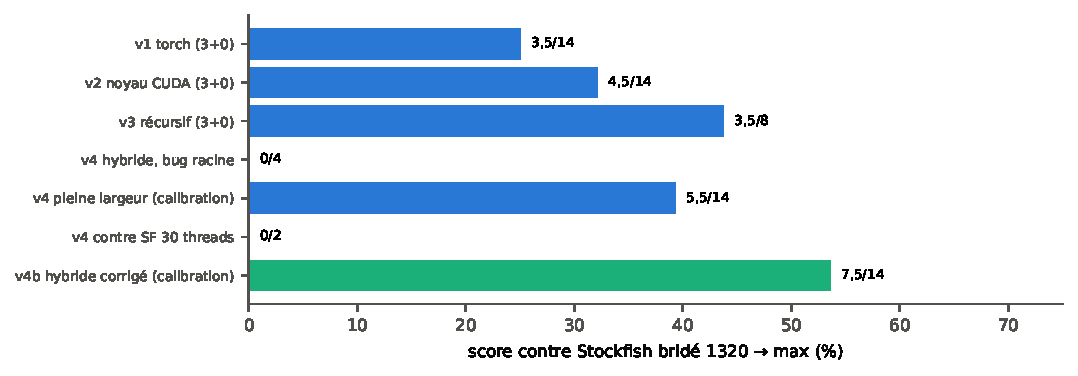
\includegraphics[width=.85\textwidth]{figs/exp_versions.pdf}
\caption{Score contre Stockfish bridé, de 1320 Elo à sa force maximale, pour chaque version du
moteur de l'incrément 1. Les versions v1 à v3 jouaient en 3+0. Les versions v4 jouaient dans les
conditions de calibration de Stockfish, soit 60~s + 0,6~s, 1 thread et 16~Mo de table.}
\end{figure}
Contre un Stockfish qui disposait de toute la machine, notre moteur visitait 1,3 fois plus de
nœuds par seconde. Stockfish atteignait pourtant 65 demi-coups, contre 7 pour nous. Son élagage
concentre la recherche sur un petit nombre de lignes.

\subsection{Fil 2 : la profondeur est le facteur limitant}
Un émulateur séquentiel du moteur a mesuré, selon la profondeur de recherche, la perte moyenne du
coup choisi par rapport au meilleur coup selon Stockfish. Cette perte passe de 71 centipions en
profondeur 4 à 20 en profondeur 8.
\begin{figure}[H]
\centering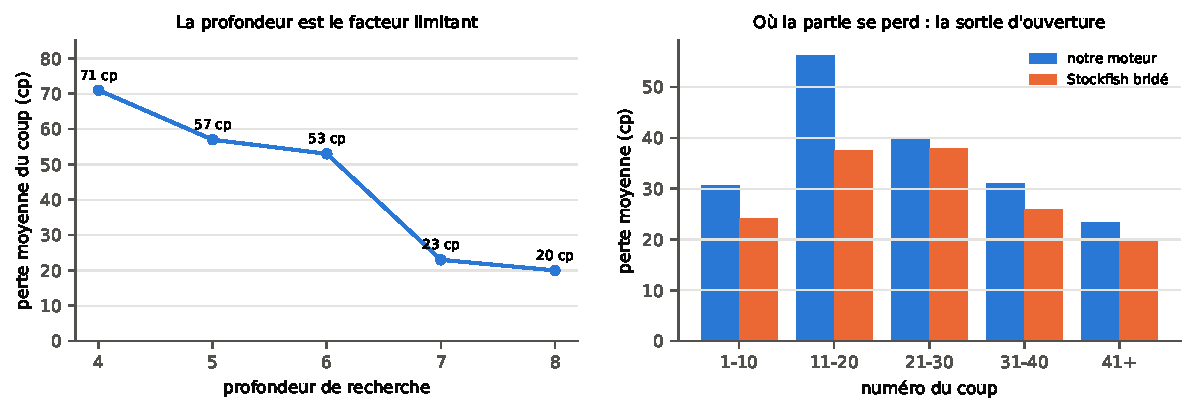
\includegraphics[width=\textwidth]{figs/exp_qualite.pdf}
\caption{À gauche, la perte par coup selon la profondeur (agent 3, incrément 1). À droite, la
perte selon le moment de la partie, mesurée par l'analyse coup par coup des 62 parties de
l'incrément 1 (incrément 2).}
\end{figure}

\subsection{Fil 3 : élaguer et trier valent plus que calculer}
Sur Kiwipete, l'alpha-bêta par lots ne visite que 0,05~\% des nœuds de la pleine largeur. À temps
égal, il gagne 2 à 3 demi-coups. En conditions de calibration, le score est passé de 5,5/14 à
7,5/14. À l'incrément 2, le tri MVV/LVA a ramené une recherche en profondeur 6 sur le gambit Dame
de 21~s à 1,1~s. Un duel de 200 parties a ensuite opposé l'ancien et le nouveau moteur, en
10~s + 0,1~s, avec des ouvertures appariées et des couleurs inversées. Le nouveau moteur marque
135/200 (67{,}5~\%), soit $+127$ Elo [$+90$ ; $+167$]
\unskip.
\begin{figure}[H]
\centering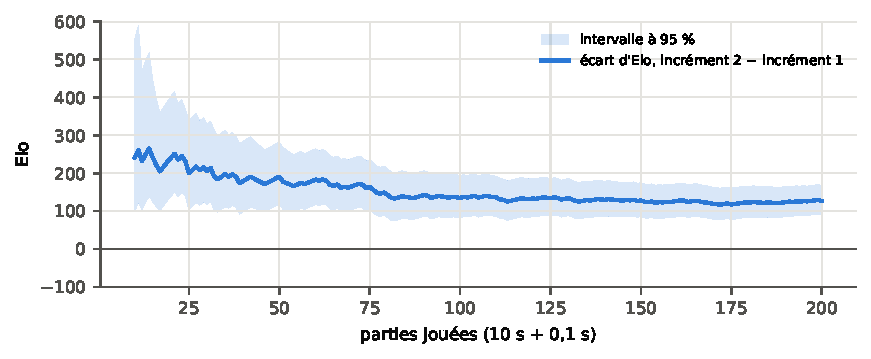
\includegraphics[width=.8\textwidth]{figs/exp_duel.pdf}
\caption{Écart d'Elo cumulé au fil du duel, avec son intervalle de confiance à 95~\%.}
\end{figure}

\subsection{Fil 4 : les parties se perdent à la sortie de l'ouverture}
L'analyse coup par coup (figure précédente, à droite) montre que notre perte moyenne passe de
31~centipions sur les coups 1 à 10 à 56 sur les coups 11 à 20, avec 5~\% de gaffes. En médiane, le
coup décisif tombe au coup 10, et c'est le nôtre dans 35 parties sur 36. Après le coup 20, l'écart
avec Stockfish bridé se réduit à quelques centipions. Le moteur perd donc ses parties à la sortie
de l'ouverture, pas en finale.

\subsection{Fil 5 : les matchs trouvent ce que les tests ratent}
Le bogue de la racine passait tous les tests de score, et seuls les matchs l'ont révélé. Deux
outils sont nés de ce constat, et le projet les lance désormais avant tout match :
\begin{itemize}
\item un \textbf{filtre de qualité} déterministe, qui mesure la perte des coups choisis, selon
Stockfish, sur 100 positions tirées avec une graine fixe ;
\item un \textbf{duel apparié}, qui donne un écart d'Elo avec son intervalle de confiance.
\end{itemize}

% =====================================================================================================
\section{Les hypothèses prometteuses}

Les cinq fils conduisent au même objectif, gagner de la profondeur utile, en particulier entre les
coups 11 et 20. Les hypothèses ci-dessous sont classées par gain attendu sur la force de jeu. Les
outils déjà en place suffisent à mesurer chacune d'elles.

\begin{hypo}{Hypothèse 1 : une table de transposition sur GPU}
Une même position peut être atteinte par plusieurs ordres de coups. Stockfish garde le résultat de
chaque recherche dans une table de transposition et le réutilise. Notre moteur cherche la position
autant de fois qu'elle apparaît. Les clés de position existent déjà (\code{position\_keys}). Une
table de hachage sur GPU, consultée par lot avant chaque vague, fournirait aussi le meilleur coup
connu pour trier la première vague.
\textbf{Mesure} : nœuds par profondeur sur les positions de \code{recherche/}, puis duel de 200
parties.
\end{hypo}

\begin{hypo}{Hypothèse 2 : une évaluation adaptée à la sortie d'ouverture}
L'évaluation actuelle ne tient compte que du matériel et de tables de position fixes. Or les plans
de coups contiennent déjà la mobilité de chaque camp, qui est le nombre de 1 du masque $(70, 64)$.
La sécurité du roi s'écrit comme les masques d'attaque, restreints au voisinage du roi. Un petit
livre d'ouvertures serait la solution la moins coûteuse.
\textbf{Mesure} : perte sur les coups 11 à 20 par l'analyse coup par coup, puis duel.
\end{hypo}

\begin{hypo}{Hypothèse 3 : l'élagage non exact, validé par duel}
Les moteurs alpha-bêta utilisent couramment deux techniques. La première réduit la profondeur des
coups tardifs (LMR). La seconde essaie d'abord de passer son tour (coup nul). Aucune des deux
n'est exacte, et le test d'égalité avec la pleine largeur ne s'applique plus. Le filtre de qualité
et le duel apparié ont été conçus pour ce cas.
\textbf{Mesure} : filtre de qualité, puis duel de 200 parties.
\end{hypo}

\begin{hypo}{Hypothèse 4 : mesurer l'Elo du moteur de l'incrément 2}
Le duel mesure un progrès relatif. Il manque une mesure absolue contre Stockfish dans ses
conditions de calibration, comme à l'incrément 1.
\textbf{Mesure} : \code{match.py -{}-preset uci-elo}, de 1320 à 2500 Elo, avec assez de parties
pour obtenir un intervalle de confiance.
\end{hypo}

\begin{hypo}{Hypothèse 5 : l'analyse rétrograde sur GPU}
La relation $b_{\text{prev}} = R\,b + c\,e_t$ se calcule avec les mêmes décalages que la marche
avant, car les pièces se déplacent de façon symétrique. Le GPU pourrait donc générer par plans les
prédécesseurs d'un lot de positions, comme il génère les coups. La rencontre au milieu deviendrait
l'intersection de deux ensembles de clés sur GPU, ce qui permettrait d'imposer une condition finale
au-delà de 3 demi-coups. On peut aussi poser le problème comme une minimisation. La valeur d'un
nœud devient sa distance au but, et l'alpha-bêta par lots sait déjà calculer un tel minimax.
\textbf{Mesure} : profondeur atteinte par \code{impose} sur les positions de \code{demo\_impose}.
\end{hypo}

\begin{hypo}{Hypothèse 6 : une contrainte en langage naturel}
Le prédicat « gagner par un mat étouffé » est déjà écrit en masques, avec un échec donné par un
cavalier et un roi entouré de ses propres pièces. Un modèle de langage pourrait traduire une
consigne en un prédicat de ce type, construit uniquement avec les fonctions existantes
(\code{attacked\_by}, \code{checker\_kinds}, voisinage du roi). Le module \code{impose} trouverait
ensuite le chemin. Le moteur vérifie que la position finale satisfait le prédicat. Il resterait à
vérifier, sur des exemples, que le prédicat traduit fidèlement la consigne.
\end{hypo}

\begin{hypo}{Hypothèse 7 : un critère de convergence pour gérer le temps}
La partie 6 a établi un critère de décision à la racine, $L(a) \ge \max_{b\ne a} U(b)$. On peut en
tirer une règle d'arrêt plus fine que la pendule, à partir de quatre signaux que le moteur mesure
déjà :
\begin{itemize}
\item l'écart $U - L$ entre le meilleur coup et le deuxième ;
\item le facteur de branchement effectif $N_d / N_{d-1}$ ;
\item le taux de coupure de la première vague (\code{Searcher.stats()}) ;
\item la stabilité du meilleur coup d'une profondeur à la suivante.
\end{itemize}
\textbf{Mesure} : temps économisé sans perte de qualité, d'après le filtre de qualité.
\end{hypo}

% =====================================================================================================
\section{Conclusion}
Les règles des échecs s'écrivent entièrement en décalages et en matrices, marche arrière comprise.
Ce calcul tourne sur une carte graphique à $5\times10^{10}$ positions par seconde. Ce débit ne
suffit pas à battre Stockfish, qui atteint 65 demi-coups là où notre moteur en atteint 7. Les deux
incréments ont montré que la force vient de la sélection des coups. L'alpha-bêta exact par lots a
fait passer le score contre Stockfish de 5,5/14 à 7,5/14. Le tri MVV/LVA, les vagues adaptatives
et la pendule de l'incrément 2 ont ajouté $+127$ Elo. Les prochaines étapes sont la table de transposition
et une meilleure évaluation à la sortie de l'ouverture. La formulation en intervalles décrit cette
sélection en termes matriciels et fournit un critère d'arrêt explicite, qui relie la génération de
coups sur GPU à la recherche.

% =====================================================================================================
\appendix
\section{Notations}
\begin{table}[H]
\centering\small
\begin{tabular}{l>{\raggedright\arraybackslash}p{8.6cm}}
\toprule
Symbole & Sens\\
\midrule
$B\in\mathbb{Z}^{8\times8}$ & plateau ; $+1$ à $+6$ du pion au roi blancs, valeurs négatives pour les noirs, 0 vide\\
$b\in\mathbb{Z}^{64}$ & plateau aplati, case $(i,j)$ à l'indice $8i+j$, a8 $=0$, h1 $=63$\\
$\shift(M, d_r, d_c)$ & décalage de $d_r$ lignes et $d_c$ colonnes, des zéros entrant par le bord\\
$E_{ab}$ & matrice $64\times64$ contenant un seul 1, en ligne $a$ et colonne $b$\\
$T = I - E_{ff} - E_{tt} + k\,E_{tf}$ & matrice d'un coup de $f$ vers $t$, de coefficient de promotion $k$\\
$R$ & matrice de retour d'un coup\\
$G = T_n\cdots T_1$ & opérateur d'une partie, stocké en étiquettes $(\mathrm{src}, \mathrm{coef})$\\
$x\in\mathbb{Z}^{94}$, $\tilde T$ & espace étendu avec cimetière, où les coups sont monomiaux\\
$(A\otimes x)_i = \max_j(A_{ij}+x_j)$ & produit dans le semi-anneau $(\max, +)$\\
$[L, U]$ & intervalle qui encadre la valeur d'un nœud\\
\bottomrule
\end{tabular}
\end{table}

\section{Glossaire}
\begin{description}
\item[Centipion (cp)] Un centième de la valeur d'un pion, unité des évaluations.
\item[Elo] Échelle de force. Un écart de 100 points donne au plus fort environ 64~\% des points.
\item[Fail-soft] Variante de l'alpha-bêta qui renvoie, quand un nœud est coupé, la borne la plus
serrée possible plutôt que $\alpha$ ou $\beta$.
\item[Kiwipete] Position de test classique de la page « Perft Results » de chessprogramming.org,
riche en roques, en prises en passant et en promotions.
\item[MVV/LVA] \emph{Most Valuable Victim, Least Valuable Attacker}. On essaie d'abord la prise de
la plus grosse pièce par la plus petite.
\item[Perft] Nombre exact de positions atteignables en $d$ demi-coups. Il sert à valider un
générateur de coups et à mesurer son débit.
\item[Quiescence] Prolongement de la recherche limité aux prises, pour ne pas évaluer une position
au milieu d'un échange.
\item[uci-elo] Nos conditions de match, qui reproduisent la calibration de Stockfish, soit
60~s + 0,6~s, 1 thread et 16~Mo de table.
\item[YBW] \emph{Young Brothers Wait}. On cherche l'aîné seul avant ses frères, pour obtenir une
fenêtre qui permettra de les couper.
\end{description}

\section{Reproduire}
Depuis la racine du dépôt :
\begin{verbatim}
python docs/etudes/2026-11-25_synthese/gen_figures.py
cd docs/etudes/2026-11-25_synthese && latexmk -pdf synthese.tex
python -m unittest src.matrix_chess.test_engine src.matrix_chess.test_retro
python -m unittest src.matrix_chess.test_gpu_engine
\end{verbatim}
Les autres documents du projet se trouvent aux emplacements suivants :
\begin{itemize}
\item le rapport de l'incrément 1 dans \code{docs/etudes/2026-11-24\_increment1-gpu/} ;
\item le rapport de l'incrément 2 dans \code{docs/etudes/2026-11-24\_increment2/} ;
\item la théorie de référence dans \code{docs/king\_matrix.md} et \code{docs/matrix\_chess.md}.
\end{itemize}

\end{document}
